\usepackage[utf8]{inputenc}
\usepackage{listings}
\usepackage{color}
\usepackage{geometry}
\usepackage[T1]{fontenc}
\usepackage[russian]{babel}
\usepackage{graphicx}

\title{Анализ бинарного файла - Lab8}
\author{Matthew Rusakov m.rusakov@innopolis.university SD-03}
\date{May 2025}



\begin{document}

    \maketitle


    \section{Введение}
    В ходе анализа был исследован бинарный файл, целью которого являлась проверка правильности введённого пользователем пароля. Программа содержит защиту от отладки (через `ptrace`) и валидирует вход только при соблюдении условий. Основной механизм верификации включает преобразование строки с помощью определённого алгоритма и сравнение результата с пользовательским вводом.


    \section{Анализ функций}

    Были исследованы следующие ключевые функции:

    \begin{itemize}
        \item FUN\_08048652 — проверка отладки и количества аргументов командной строки.
        \item FUN\_080485a5 — валидация, что строка состоит только из цифр, шифрование строки "THEPASSWORDISEASYTOCRACK" и сравнение с пользовательским вводом.
        \item FUN\_0804851c — функция, шифрующая исходную строку.
        \item FUN\_080484f4 — функция, копирующая строку без завершающего нуля.
    \end{itemize}


    \section{Основные моменты}

    \begin{itemize}
        \item Пароль должен состоять только из цифр.
        \item Сравнение происходит между результатом шифрования строки "THEPASSWORDISEASYTOCRACK" и пользовательским вводом.
        \item Реализация FUN\_0804851c содержит несколько операций XOR и математических преобразований по каждому байту.
    \end{itemize}


    \section{Шифратор}

    Шифратор на языке Python, для генерации правильного пароля:

    \begin{verbatim}

        def encrypt_password(input_str: str) -> str:
            data = bytearray(input_str.encode('utf-8'))

            data[0] ^= 0xAB

            for i in range(1, len(data)):
                data[i] = (data[i] - i) & 0xFF
                data[i] ^= data[i - 1]
                data[i] = (data[i] + data[i - 1]) & 0xFF
                data[i] ^= data[i - 1]
                data[i] ^= data[8] if len(data) > 8 else 0
                if data[i] == 0:
                    data[i] = 1

            return ''.join(f"{byte:02x}" for byte in data)


        if __name__ == "__main__":
            plaintext = "THEPASSWORDISEASYTOCRACK"
            encrypted = encrypt_password(plaintext)
            print(f"Encrypted result: {encrypted}")

    \end{verbatim}


    \section{Тестовый запуск}


    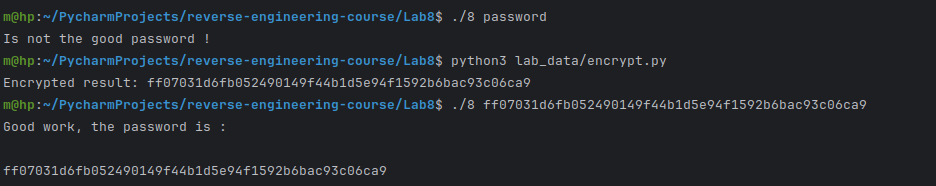
\includegraphics[width=1\linewidth]{lab_data/solution}


    \section\*{Вывод}

    Анализ показал, что программа использует собственный способ шифрования строки и проверяет, соответствует ли
    пользовательский ввод результату этого шифрования.
    Далее я реализовал питоновский скрипт, который позволяет получить правильный пароль.

    Правильный пароль: ff07031d6fb052490149f44b1d5e94f1592b6bac93c06ca9

    \begin{thebibliography}{1}
        \bibitem{githublink}
        GitHub Link: https://github.com/MattWay224/reverse-engineering-course
        В этом репозитории можно найти все лабы и информацию про каждое задание в каждой лабе
    \end{thebibliography}
\end{document}
